
\section{Background}\label{sec:Background}

\subsection{Routing loops in DCNs}\label{subsec:loop}

Various loop incidents have been observed in both Google's and Microsoft's production DCNs~\cite{libra,everflow}. In DCNs, routing loops arise when there are inconsistencies in routing state among a set of switches. Routing inconsistencies can be caused by many network errors including corruption of forwarding entries, failure of devices and misconfiguration of network devices.

Routing loops can be either persistent or transient. Persistent loops are commonly caused by misconfiguration or device bugs, and require human intervention to fix them. Transient loops arise as different switches in a network usually converge at different speed when a network failure occurs. The duration of a transient loop is directly related to the convergence time of the routing protocol in use. The convergence times of different routing protocols, e.g., BGP~\cite{bgp}, are different and are affected by the network scale.

\subsection{Priority-based Flow Control in RDMA DCNs}\label{sec:rdma_dcns}


Driven by the rising demand of cloud applications, we are deploying RoCEv2-based RDMA in Microsoft's DCNs to provide ultra-low latency (10us per hop or less) and high throughput (40Gbps or more), with very low CPU overhead. The deployment of RoCEv2-based RDMA needs Priority-based Flow Control (PFC) to enable a lossless Ethernet fabric~\cite{dcqcn}. When a switch port or a NIC is unable to accommodate more packets in its buffer, PFC can prevent buffer overflow by sending PAUSE frames to its directly connected upstream device to stop further data transmission.

%RDMA can enable the network interface cards (NICs) to transfer data directly to or from application memory without any operating system involvement and thus reduce both CPU overhead and overall latency.
In more details, switches and NICs track the queue length of each ingress queue\footnote{Packets are actually only buffered in the egress queues, but the device will maintain a counter to track the queue length of each virtual ingress queue.}. Once the queue length exceeds a certain threshold, a PAUSE frame will be sent to the upstream device. The upstream device then stops transmission on that link for some amount of time specified in the PAUSE frame or until receive a RESUME frame from its downstream device.

PFC has a cascade effect: Once a link is paused for a long time due to traffic congestion, related interfaces of upstream devices will be paused hop-by-hop backward until traffic sources are finally paused. This cascade effect will not be a problem if PFC can operate at a per flow level. However, due the the hardware limitation, PFC now operates at a per port (or, port plus priority) level and can at most support 8 priority classes, which means that a flow is possible to be paused by a congested link that is not even on its path.

The using of PFC mainly introduces two problems: congestion spreading problem and deadlock problem.

Under normal circumstances (i.e., no network error happens), congestion spreading problem can be well handled by running an effective flow-level congestion control protocol at all server NICs, e.g., DCQCN~\cite{dcqcn} is such an protocol we have designed for our RoCEv2-based RDMA DCNs. But in practice, it is difficult to guarantee that the network will never run into any incorrect state, especially for large scale DCNs consists of tens of thousands of switches and millions of servers. We found that the behaviour of PFC is dangerous when the network is in an incorrect state. With PFC, even a transient routing loop is possible to bring the whole DCN into a permanent deadlock state. More details will be introduced in the next part.
%
%\subsection{Deadlock problem in RDMA DCNs}\label{sec:deadlock_problem}
%
%In this part, we introduce several deadlock cases that have been observed in our production data centers.

%\subsubsection{Routing loop induced deadlock}\label{subsec:loop_deadlock}
%
%
%
%\parab{Routing loops in DCNs:}  In the next, we use a small three-level Clos network to illustrate three loop scenarios caused by different network errors.
%
%\begin{figure}[t]
%\centering
%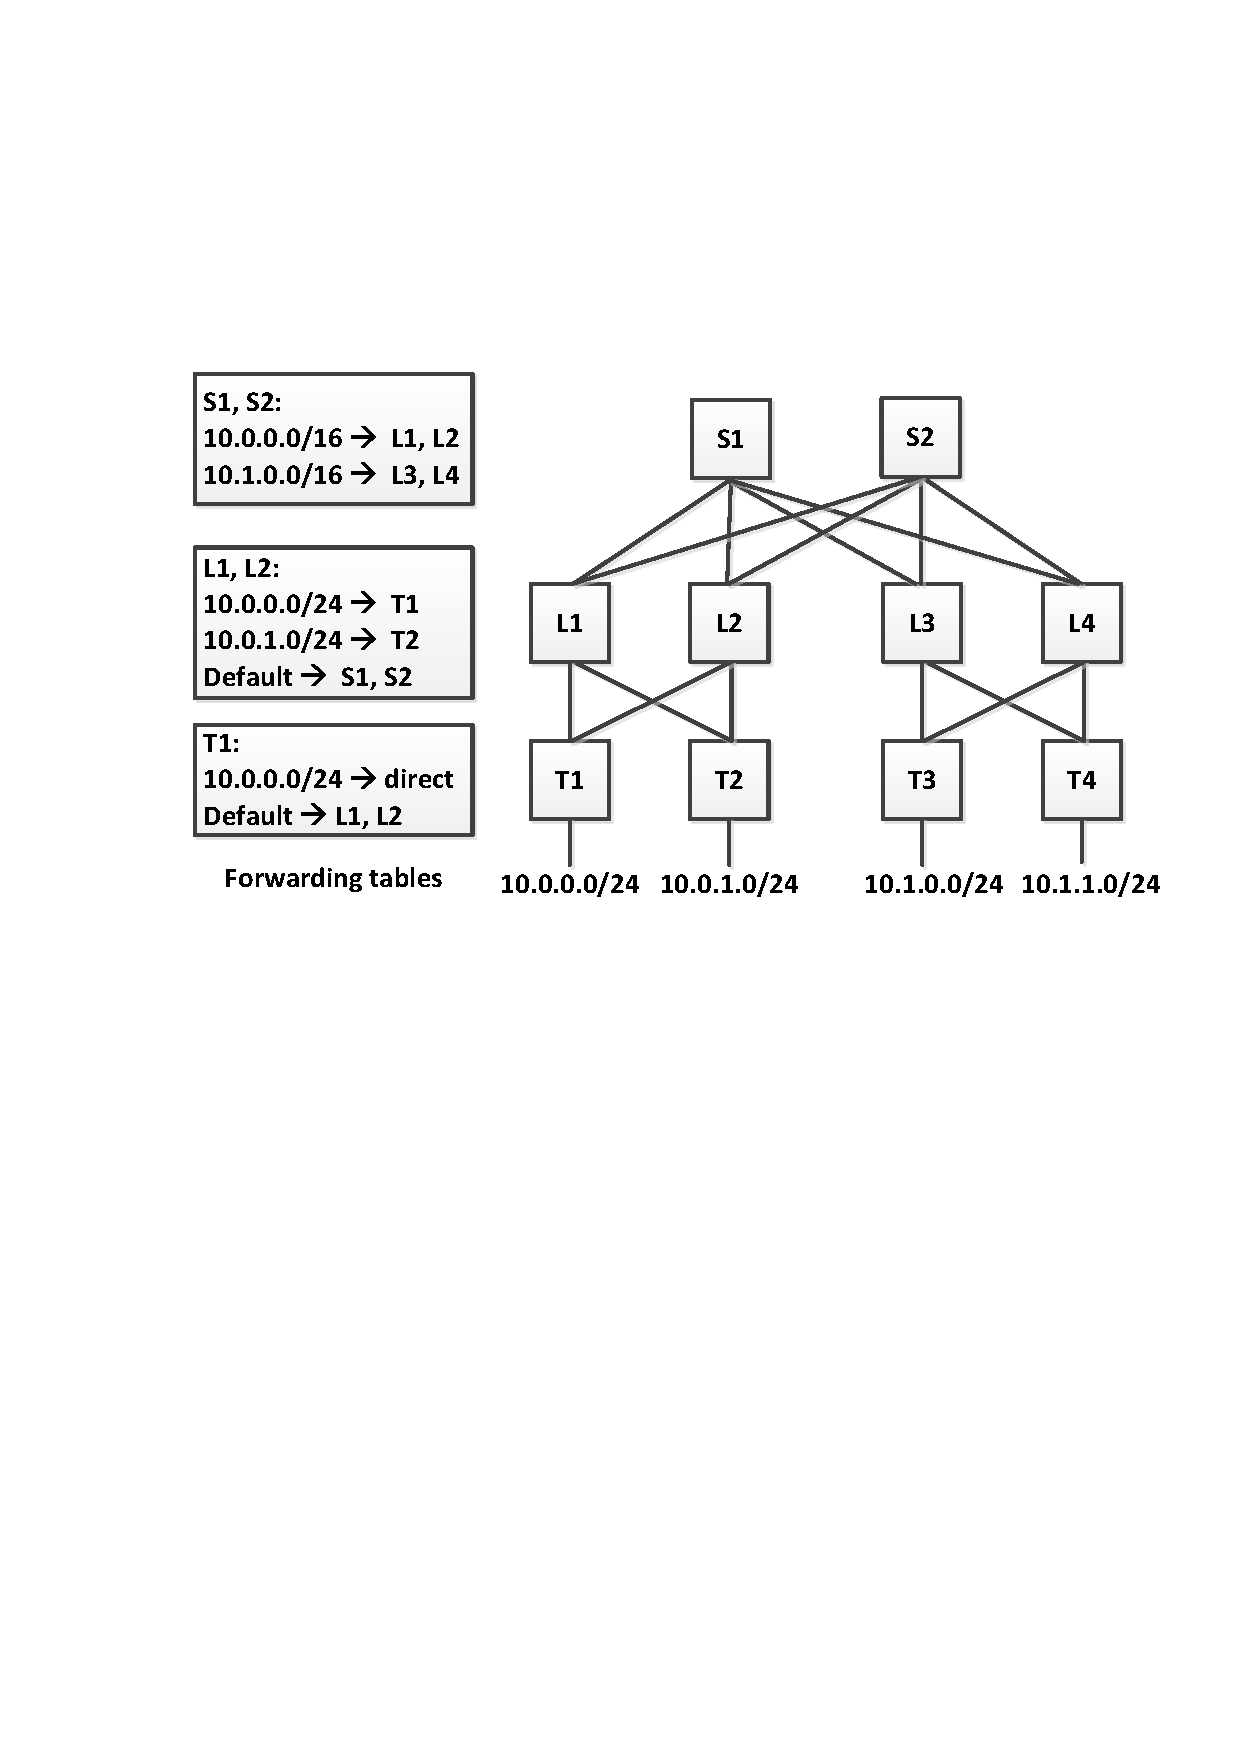
\includegraphics[width=0.5\textwidth,center]{figs/loop_example_a.pdf}
%\caption[Optional caption for list of figures]{A three-level Clos network for illustrating routing loops.}
%\label{fig:routing_loop}
%\end{figure}
%
%A three-level Clos network consisting of 10 switches is shown in Fig.~\ref{fig:routing_loop}. In the topology, each ToR switch is directly connected to a set of servers in some subnet, e.g., servers in subnet "10.0.0.0/24" are directly connected to switch T1. The forwarding tables drawn in Fig.~\ref{fig:routing_loop} are the correct ones when the network is in a correct state. Note that ECMP (equal cost multipath) is used to do traffic load-balancing across all paths in the network.

%\begin{figure}[t]
%\centering
%%\vspace{-0.15in}
%\subfloat[short for lof][Loop caused by mis-configuration.] {
%    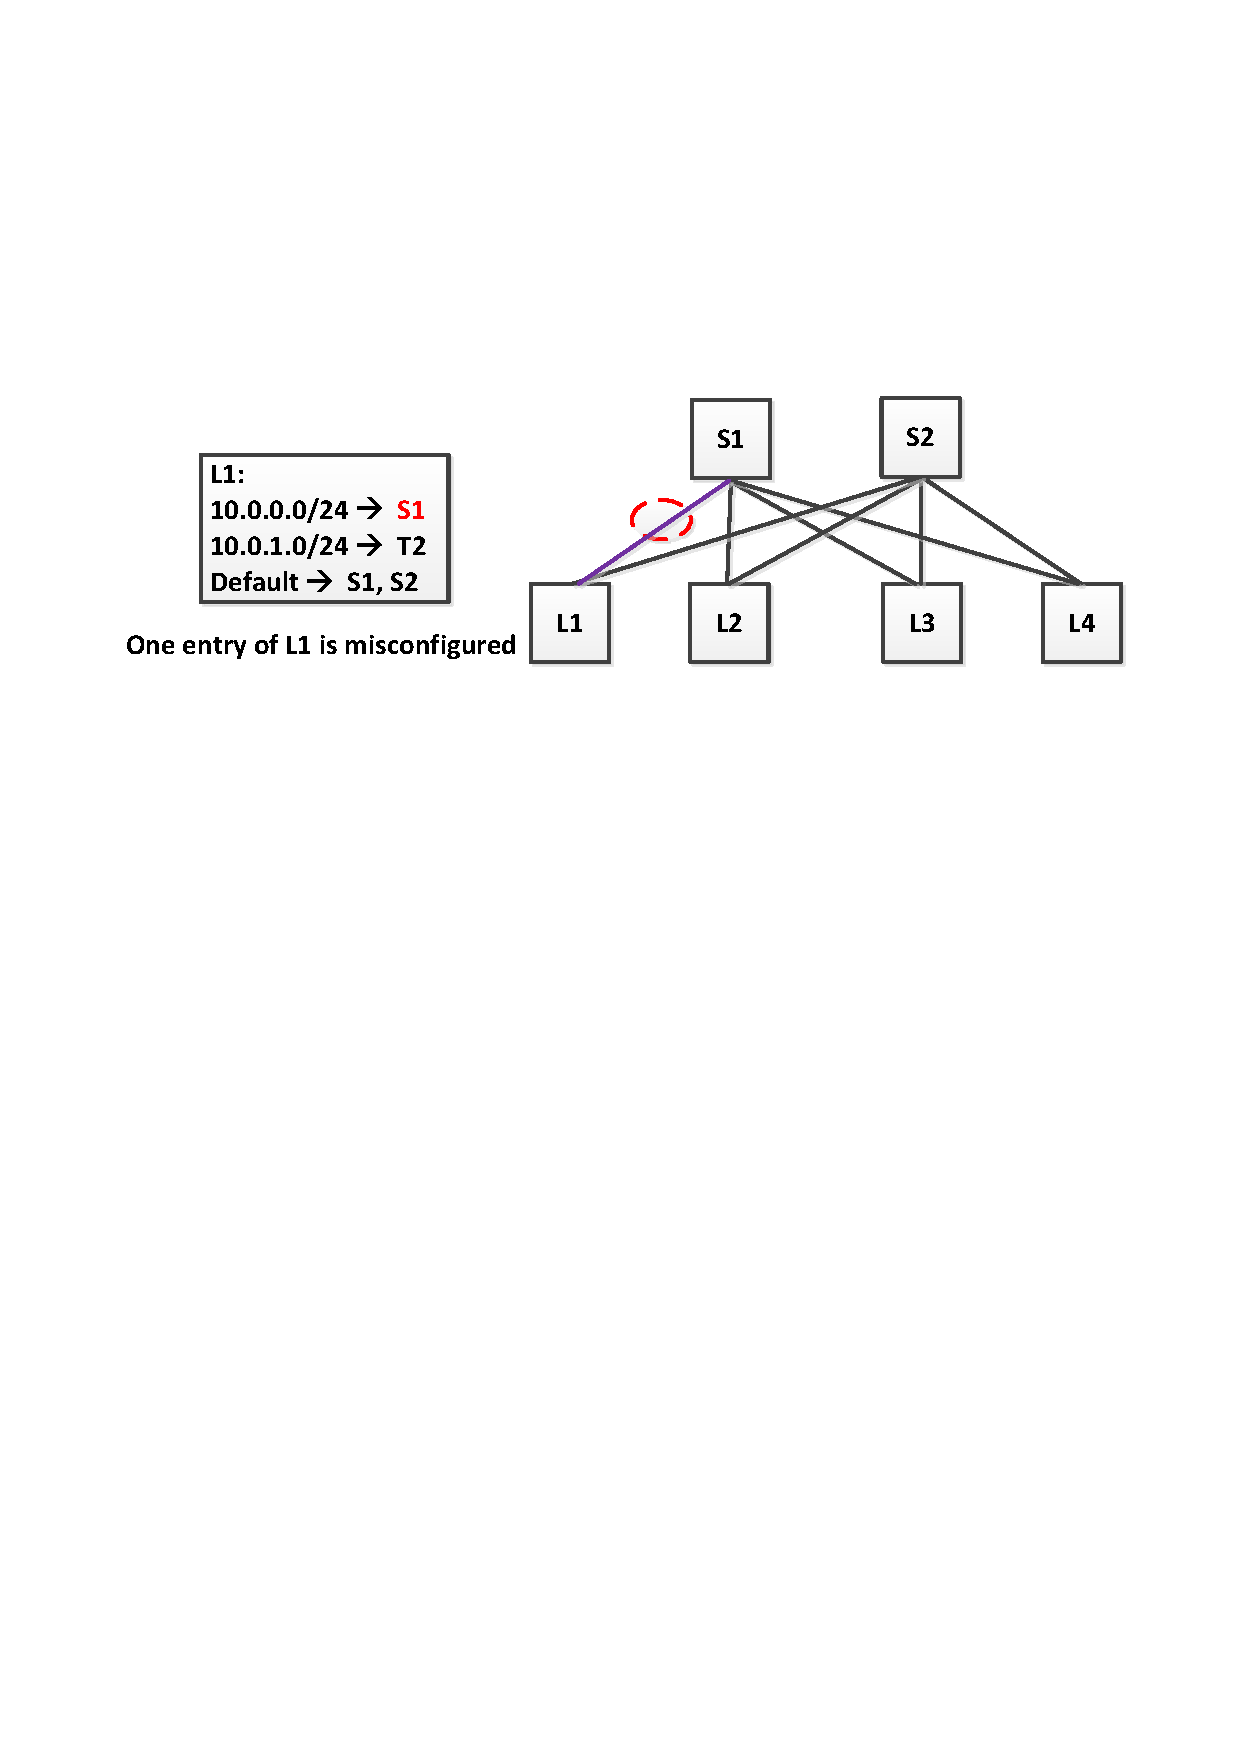
\includegraphics[width=0.5\textwidth] {figs/loop_example_b.pdf}
%    \label{fig:network-update_a}
%}
%
%%\vspace{-0.15in}
%\subfloat[short for lof][Loop caused by entry corruption.] {
%    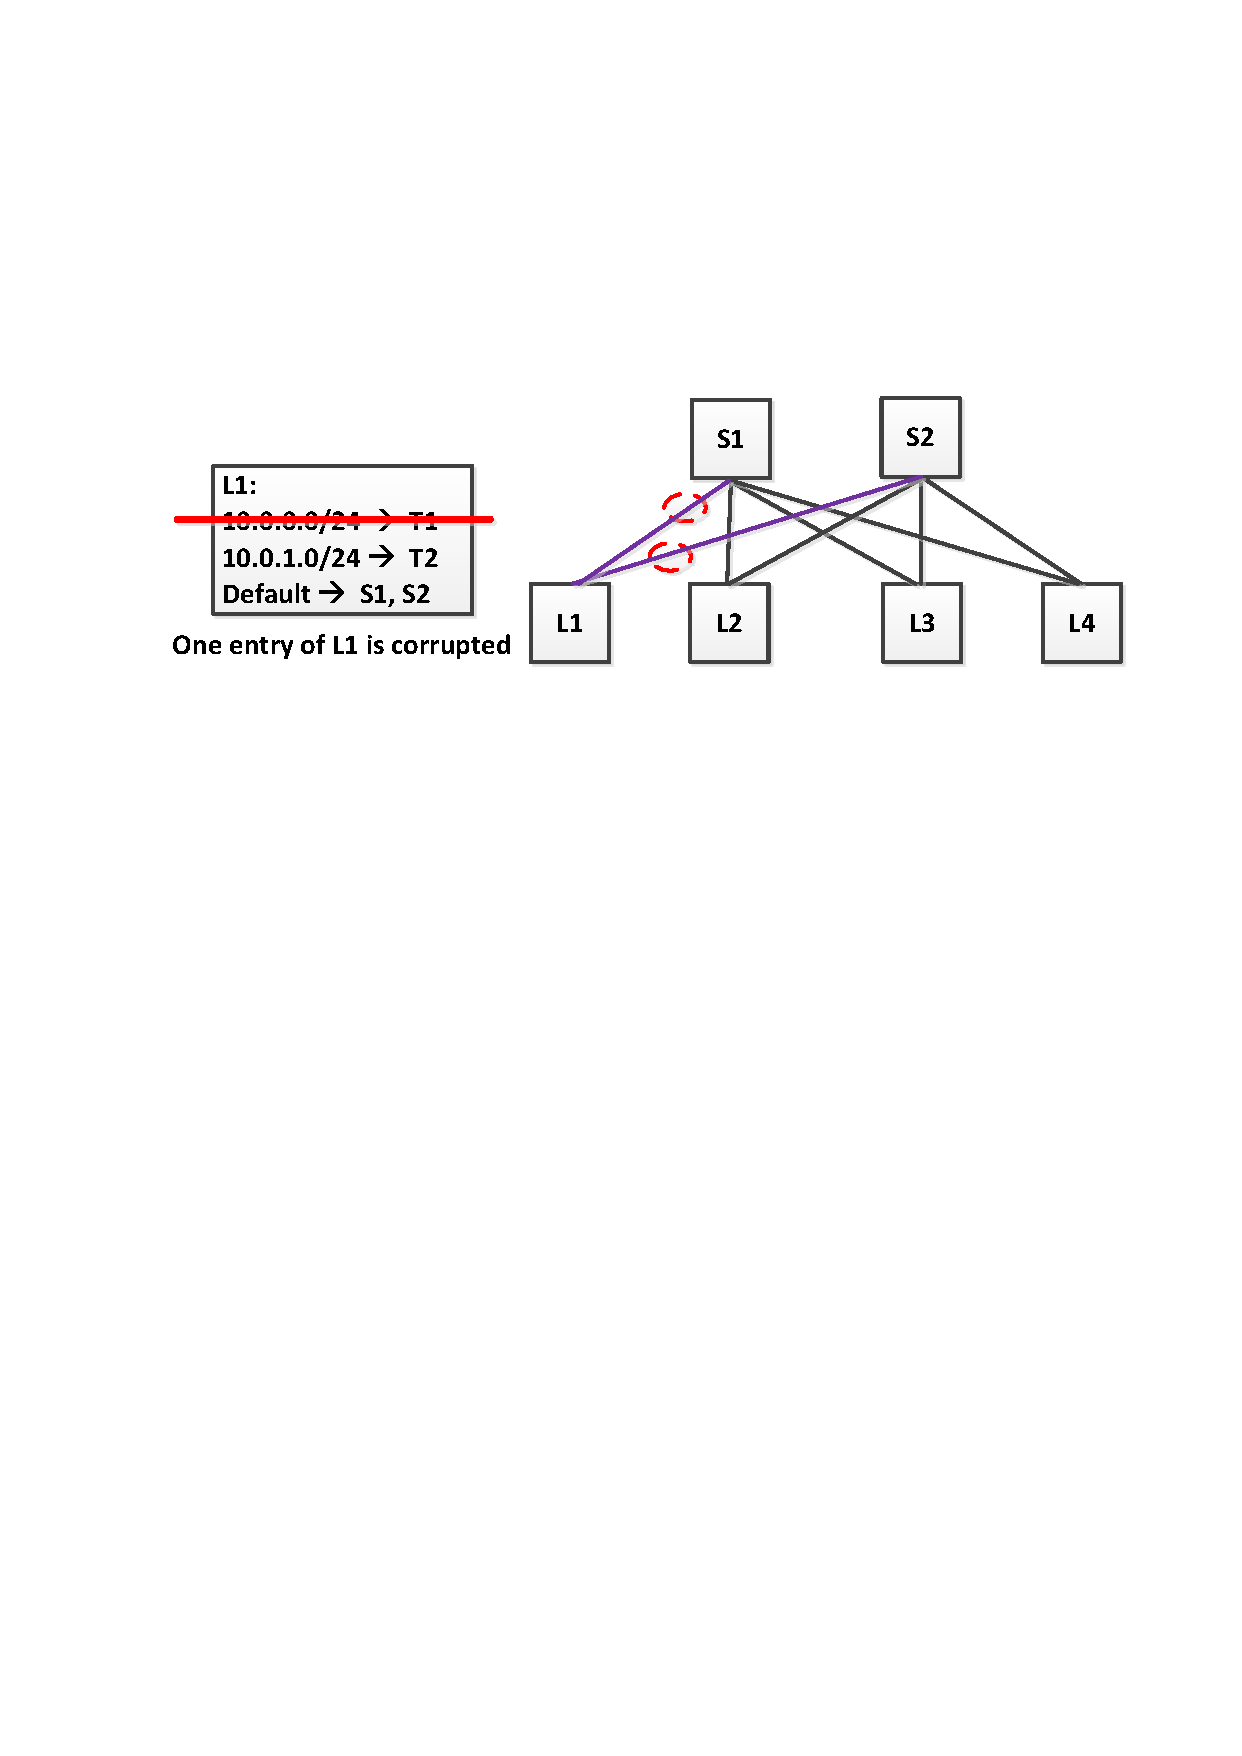
\includegraphics[width=0.5\textwidth] {figs/loop_example_c.pdf}
%    \label{fig:network-update_a}
%}
%
%\subfloat[short for lof][Loop caused by switch failure.] {
%    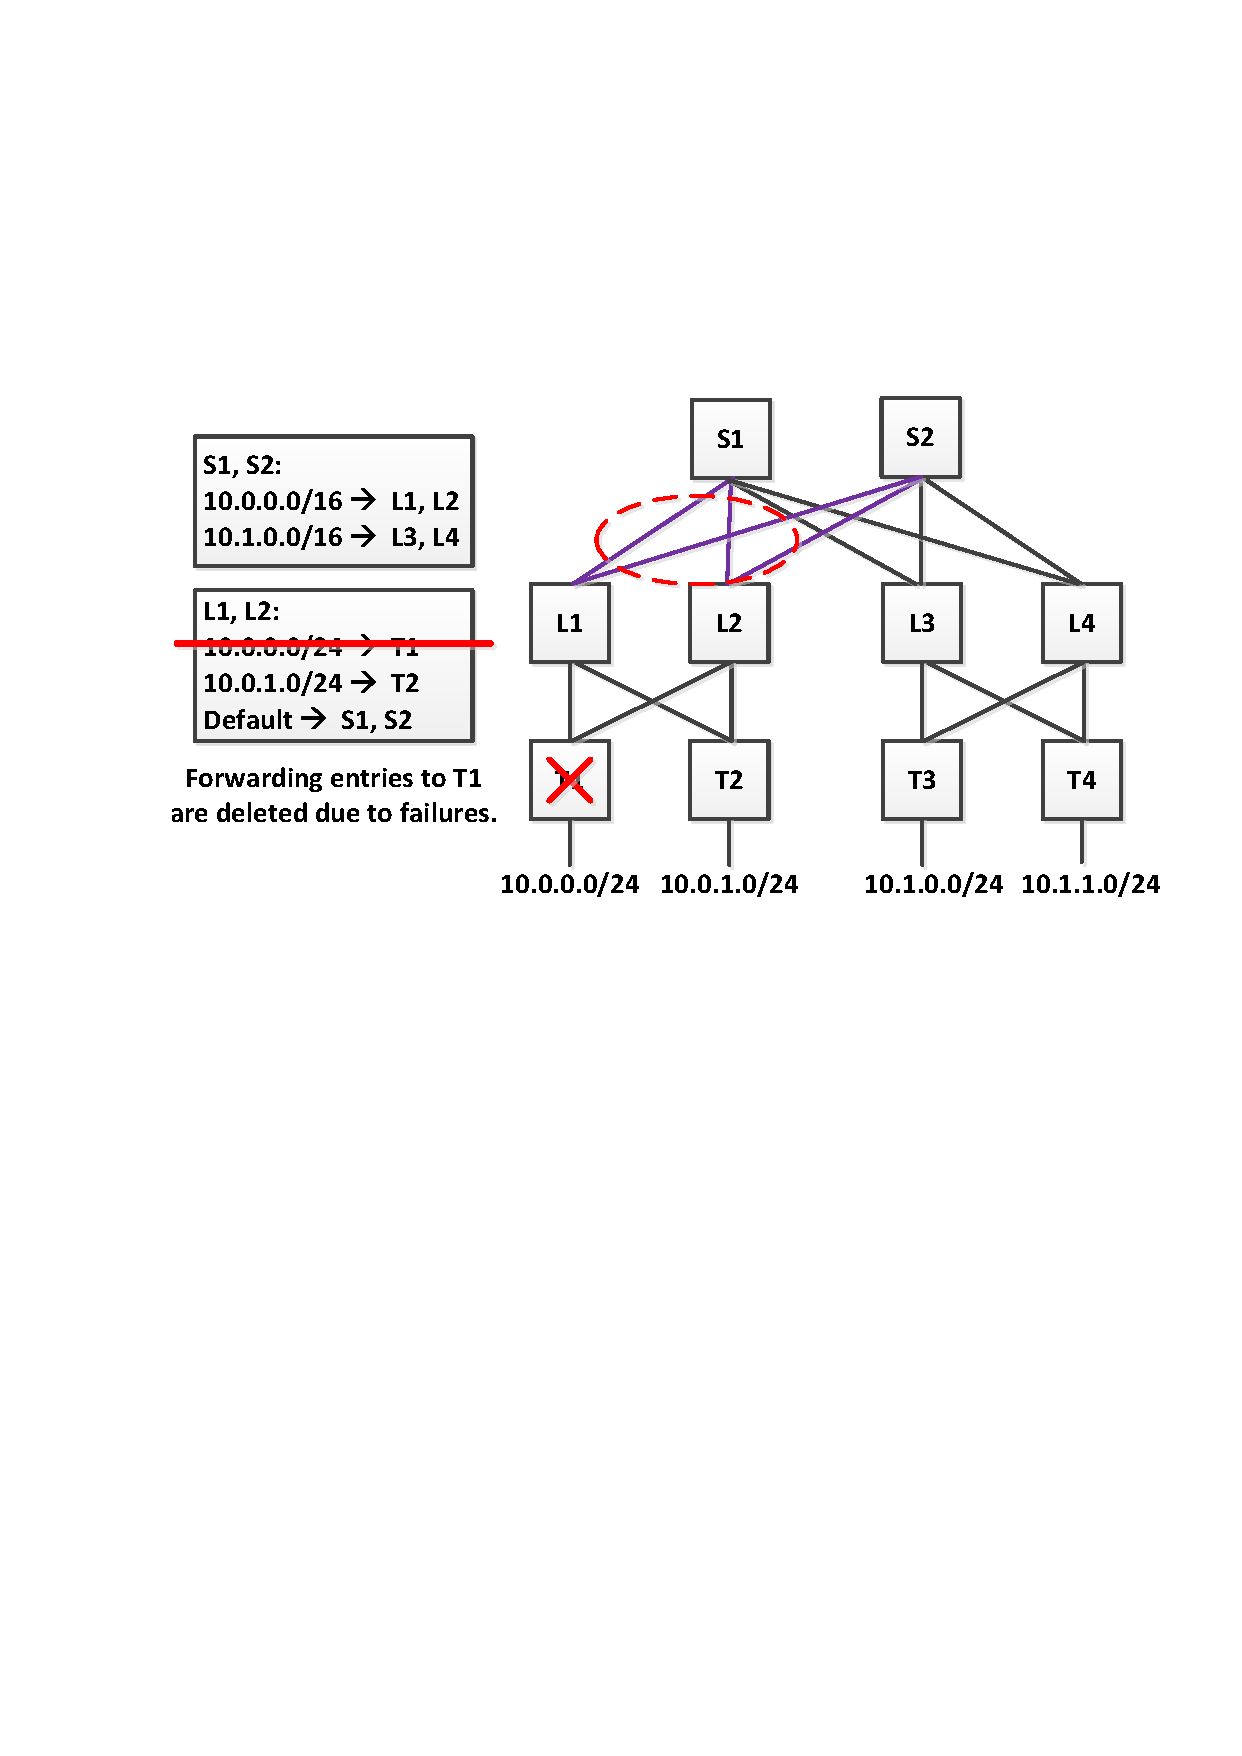
\includegraphics[width=0.5\textwidth] {figs/loop_example_d.pdf}
%    \label{fig:network-update_a}
%}
%%\vspace{-0.1in}
%\caption[Optional caption for list of figures]{Three loop scenarios caused by different network errors.}
%\label{fig:loop_scenarios}
%%\vspace{-0.2in}
%\end{figure}
%
%Fig.~\ref{fig:loop_scenarios}(a) shows how a switch mis-configuration causes a loop. Due to a mis-configuration, the forwarding entry "10.0.0.0/24 $\rightarrow$ T1" becomes "10.0.0.0/24 $\rightarrow$ S1".  This creates a loop "S1 $\rightarrow$ L1 $\rightarrow$ S1" for the packets destined for the subnet "10.0.0.0/24".
%
%Fig.~\ref{fig:loop_scenarios}(b) shows how a entry corruption causes two loops. In this scenario, the entry ``10.0.0.0/24 $\rightarrow$ T1" becomes invalid due to the entry corruption in the TCAM table. Then all the traffic destined for subnet ``10.0.0.0/24" will be forwarded back to either switch S1 or switch S2 by the default route ``Default $\rightarrow$ S1, S2". This creates two loops: ``S1 $\rightarrow$ L1 $\rightarrow$ S1" and ``S2 $\rightarrow$ L1 $\rightarrow$ S2".
%
%Fig.~\ref{fig:loop_scenarios}(c) shows that a switch failure can also cause routing loops. In this scenario, switch T1 is down due to some failure. After detecting the failure of its neighbor, Switches L1 and L2 will delete the entry ``10.0.0.0/24 $\rightarrow$ T1" and stop forwarding packets to switch T1. However, Switch S1 and S2 will still forward packets destined for subnet ``10.0.0.0/24" to either L1 or L2 as they are not aware of the failure of switch T1. Then the packets will be forwarded back to S1 or S2 by the default entry ``Default $\rightarrow$ S1, S2". Three loop are created in this scenario: ``S1 $\rightarrow$ L1 $\rightarrow$ S1", ``S2 $\rightarrow$ L1 $\rightarrow$ S2" and ``S1 $\rightarrow$ L1 $\rightarrow$ S2 $\rightarrow$ L2 $\rightarrow$ S1".
%
%
%%The adoption of dynamic routing protocols such as BGP and OSPF can help the network to recover from routing loops automatically. The convergence time
%
%
%\subsubsection{Device bug induced deadlock}\label{subsec:bug_deadlock}
%\todo{to be added.}
